%==============  code_only_box.tex  =================
\documentclass[11pt]{article}

% 레이아웃/폰트 (필요 없으면 빼도 됨)
\usepackage{geometry}
\geometry{margin=1in}
\usepackage{fontspec}
\usepackage[space]{xeCJK}          % ← minted와의 verbatim 충돌 피하려면 [space] 옵션은 쓰지 마세요
\setCJKmainfont{Noto Sans KR}

\usepackage{setspace}
\setstretch{1.2}
\setlength{\parindent}{0pt}
\setlength{\parskip}{6pt}

% tcolorbox + (minted|listings) 토글
\newif\ifuseminted
\usemintedtrue             % minted 사용(하이라이트 예쁨). 안 되면 false로 바꿔 listings 사용

\usepackage[many]{tcolorbox}
\tcbuselibrary{skins,breakable,listings,minted}
\usepackage{xcolor}
\definecolor{codebg}{RGB}{248,248,248}
\usepackage{enumitem}          % ★ 필요
\usepackage{graphicx}
% --- minted 버전: "코드 전용" 박스 (listing only)
\ifuseminted
  \usepackage{minted}       % 컴파일: xelatex -shell-escape code_only_box.tex
  \newtcblisting{CodeBox}[1][]{
    enhanced, breakable,
    colback=codebg, frame hidden,
    boxrule=0pt, borderline={0.5pt}{0pt}{black!15, dashed},
    sharp corners, before skip=8pt, after skip=12pt,
    listing engine=minted,
    listing only,            % ★ 박스 안엔 오직 코드만
    minted language=python,  % 필요 시 \begin{CodeBox}[minted language=c++] 로 덮어쓰기
    minted options={
      fontsize=\small,
      breaklines,
      autogobble,
      linenos,
      numbersep=6pt,
      tabsize=2
    },
    #1                       % 사용자 옵션 전달
  }
\else
% --- listings 버전: shell-escape 불가 시
  \usepackage{listings}
  \lstdefinestyle{mylist}{
    basicstyle=\ttfamily\small,
    numbers=left, numbersep=6pt,
    breaklines=true,
    tabsize=2,
    backgroundcolor=\color{codebg},
    showstringspaces=false
  }
  \newtcblisting{CodeBox}[1][]{
    enhanced, breakable,
    colback=codebg, frame hidden,
    boxrule=0pt, borderline={0.5pt}{0pt}{black!15, dashed},
    sharp corners, before skip=8pt, after skip=12pt,
    listing engine=listings,
    listing only,            % ★ 박스 안엔 오직 코드만
    listing options={style=mylist, language=Python},
    #1
  }
\fi



\begin{document}

\begin{center}
  {\LARGE \bfseries FMOVQE 코드 주석 정리} \\[10pt]
  {\large 최윤호}
\end{center}

\section{사전 정의 함수}
\subsection{최적화 정보 저장 함수}
% 박스 안: 원문 코드만
\begin{CodeBox}[title={Example: Python snippet}]
def make_intermediate_info():
    intermediate_info = {
        'nfev ': [], 
        'parameters ': [],
        'energy ': [],
        'stddev ': []
    }
def callback (nfev , parameters , energy , stddev ):
    intermediate_info ['nfev ']. append ( nfev )
    intermediate_info ['parameters ']. append ( parameters )
    intermediate_info ['energy ']. append ( energy )
    intermediate_info ['stddev ']. append ( stddev )
\end{CodeBox}

\begin{enumerate}[label=\textbf{*}, leftmargin=*]
  \item nfev : 목적함수를 몇번 불러왔는가.( = Iteration의 횟수 )
  \item parameters : 최적화 과정에서 사용된 파라미터
  \item energy : 에너지 계산결과 (목적함수의 결과값)
  \item stddev : 에너지 계산과정이 여러번의 측정을 통한 통계적 계산이므로, 그때 생기는 표준편차. 
\end{enumerate}
그리고 이를 이용하여 callback 함수를 정의. 이후 계산에서는 energy에 해당하는 값만 사용. 
\subsection{Exact Solver}
\begin{CodeBox}[title={Example: Python snippet}]
def exact_solver(qubit_op, problem):
    sol = NumPyMinimumEigensolver().compute_minimum_eigenvalue(qubit_op)
    result = problem.interpret(sol)
    return result
\end{CodeBox} 
파울리 스트링으로 저장되어있는 헤밀토니안인 "qubit\_op"를 받아서. 이를 대각화 하여 가장 작은 고유값을 계산한다. 
"qubit\_op"의 경우 아래와같은 SparsePauliOp의 형태로 파울리 스트링의 선형결합으로 저장되어있다. 
\begin{CodeBox}[title={Example: Python snippet}]
SparsePauliOp(['IIII', 'IIIZ', 'IIZI', 'IIZZ', 'IZII', 'IZIZ', 'ZIII', 'ZIIZ', 'YYYY', 'XXYY', 'YYXX', 'XXXX', 'IZZI', 'ZIZI', 'ZZII'],
coeffs=[-0.81054798+0.j,  0.17218393+0.j, -0.22575349+0.j,  0.12091263+0.j,0.17218393+0.j,  0.16892754+0.j, -0.22575349+0.j,  0.16614543+0.j, 0.0452328 +0.j,  0.0452328 +0.j,  0.0452328 +0.j,  0.0452328 +0.j, 0.16614543+0.j,  0.17464343+0.j,  0.12091263+0.j])
\end{CodeBox} 

\subsection{파울리 매핑}
\begin{CodeBox}[title={Example: Python snippet}]
def fermion_to_qubit(problem, second_q_op, mapper_name):
  if mapper_name == "JW":
    mapper = JordanWignerMapper()
  if mapper_name == "Pa":
    mapper = ParityMapper(num_particles=problem.num_particles)
  if mapper_name == "BK":
    mapper = BravyiKitaevMapper()
  qubit_op = mapper.map(second_q_op)

  return qubit_op , mapper
\end{CodeBox} 
\begin{enumerate}[label=\textbf{*}, leftmargin=*]
  \item mapper\_name: "JW", "Pa", "BK" 등의 사용할 매핑방식의 약자
  \item Problem : 전자수, 오비탈수 등 분자의 여러 정보들을 담고있는 클래스
  \item Second\_q\_op : 생성/소멸 연산자로 구성되어있는 헤밀토니안
\end{enumerate}
mapper\_name 으로 정의된 매핑방식을 이용하여 Second\_q\_op 를 앞서 사용한 qubit\_op 의 형태로 매핑한다. 이떄 Parity 매핑방식에는 up-spin 전자와 down-spin 전자의 개수에 대한 정보가 필요하므로, 이를 problem 으로부터 problem.num\_particle 을 통해 가져온다. 

problem.num\_particle = (up-spin 전자수, down-spin 전자수) 인 튜플

\newpage

\section{에너지 계산 함수}
\begin{CodeBox}[title={Example: Python snippet}]
def least_Energy(as_problem):
    # as_problem :ActiveSpaceTransformer를 통해 힐버트 공간을 줄인 Dirver
    as_num_particles = as_problem.num_particles
    # (up-spin 전자수, down-spin 전자수) 인 튜플
    as_num_spatial_orbitals = as_problem.num_spatial_orbitals
    # 시스템의 spatial orbital 갯수
    as_fermionic_hamiltonian = as_problem.hamiltonian
    # 시스템의 헤밀토니안 (여러가지의 형태로 헤밀토니안이 정의되어있음)
    as_second_q_op = as_fermionic_hamiltonian.second_q_op()
    # 그중 생성/소멸 연산자로 정의된 헤밀토니안
    energy_arr = [] 
    # 각 Ansatz, optimizer 별 최종 수렴 에너지를 저장할 리스트
    ansatz_order = [] 
    # 그래프의 제목을 위해 for 문에서 사용한 Ansatz 순서를 기록하기 위한 리스트
    opt_order=[]
    # 그래프의 제목을 위해 for 문에서 사용한 optimizer 순서를 기록하기 위한 리스트
    qubit_op, mapper = fermion_to_qubit(as_problem, as_second_q_op, "Pa")
    # 사전에 정의한 함수 "fermion_to_qubit"을 통해 생성/소멸 연산자로 정의된 헤밀토니안인 as_second_q_op 를 파울리 스트링으로 매핑
    as_init_state = HartreeFock(as_num_spatial_orbitals,as_num_particles,mapper)
    # 파동함수를 나타내기 위한 초기상태, 특히 UCCSD 에서는 1차여기와 2차여기 연산자들이 가해질 Reference State가 되는 초기상태를 정의. 여기서는 HartreeFock 함수를 통해 생성.
    # HartreeFock 상태에서는 Qiskit에서 오비탈을 정렬하는 정의에 의해, (up-spin 전자수, down-spin 전자수) 만큼 앞의 오비탈이 1인 상태 
    uccsd = UCCSD(as_num_spatial_orbitals,as_num_particles,mapper,initial_state=as_init_state, generalized=True)
    # UCCSD Ansatz 를 Qiskit 에서 제공하는 패키지를 이용해 정의. 
    # generalized 옵션은 임의의 오비탈에서의 전이를 허용하여 계산량은 늘어나지만, 높은 표현력을 얻을 수 있음 
    twolocal = TwoLocal(as_num_spatial_orbitals*2, ['ry', 'rz'], 'cz', initial_state=as_init_state)
    # twolocal Ansatz 를 Qiskit 에서 제공하는 패키지를 이용해 정의.
    # spin orbital 만큼의 큐비트가 필요하므로, 공간오비탈의 개수에 2배를 해준다. 
    # Rotation Gate는 'ry', 'rz' 를 사용. 
    # Entanglement는 'cz' 를 이용해 표현 
    ansatzs=[uccsd,twolocal]
    # 여러 Ansatz 와 optimizer 에 대해서 실험을 하기위해 각 구성에 대한 리스트를 구성
    iter = [250,1000]
    # Ansatz 별로 각 Iteration에서 소요되는 시간이 다르므로 두개의 max_iter를 정의
    ansatzs_name=['UCCSD','Two local']
    # 이때 Ansatz 는 해당 양자회로를 리스트로 만들었으므로, 그림을 그리는데에 필요한 이름 리스트 또한 만들어준다. 
    opt_names = ['COBYLA','SPSA','L-BFGS-B'] 
    # optimizer는 VQE 함수에서 스트링으로 옵션을 주게 되므로, 따로 만들지 않아도 괜찮다. 
    noiseless_estimator = Estimator()
    # 구버전인 Qiskit Primitive 에서 제공하는 Estimator를 정의 이때 backend도 같이 시뮬레이터로써 정의됨. 
    for i in range(2): # 2개의 Ansatz 계산을 위한 for문
        ansatz = ansatzs[i]
        ansatz_name= ansatzs_name[i]
        MAX_ITER = iter[i]
        # i(0 또는 1)번째 Ansatz가 이번 for문에서 사용될 Ansatz임을 정의 
        opt_arr = [COBYLA(maxiter=MAX_ITER),SPSA(maxiter=MAX_ITER),L_BFGS_B(maxiter=MAX_ITER)]
        # 3개의 optimizer 에 대한 리스트 생성
        for k in range(3): # 3개의 optimizer 에 대한 계산을 위한 for문
        #즉, 이 밑의 계산이 총 6번 진행된다.
            make_intermediate_info()
            # callback 함수의 딕셔너리를 초기화
            optimizer = opt_arr[k]
            opt_name = opt_names[k]
            # k(0,1 또는 2)번째 optimizer가 이번 for문에서 사용될 optimizer임을 정의 
            vqe = VQE(noiseless_estimator, ansatz, optimizer, callback = callback)
            # 초기에 실험했던 함수로써 Qiskit 에서 제공하는 VQE 함수를 사용 
            # 위에서 정의한 변수들을 이용하여 VQE 계산을 정의
            result = vqe.compute_minimum_eigenvalue(qubit_op)
            # vqe.compute_minimum_eigenvalue 함수를 통해 qubit_op 라는 파울리 스트링으로 표현된 헤밀토니안에 대한 바닥상태 에너지를 계산.
            vqe_result = result.eigenvalue.real
            # 계산된 결과인 가장 작은 eigenvalue를 실수값으로 반환
            core = as_problem.hamiltonian.constants['ActiveSpaceTransformer']
            # ActiveSpace 를 정의할때 core space로 무시한 오비탈 들에대한 에너지 계산 (상수)
            repulsion = as_problem.hamiltonian.constants['nuclear_repulsion_energy']
            # Born-oppenheimer 근사를 적용할때 상수로 처리되었던 핵간 척력을 계산 (상수)
            
            exact_energy = exact_solver(qubit_op, as_problem).total_energies[0].real
            # 헤밀토니안을 직접 대각화 하여 Exact한 결과를 계산
            dimer_energy = vqe_result+repulsion + core
            # VQE 의 결과와 Core 오비탈의 에너지, 핵간 척력 에너지를 더하여 최종결과 계산
            Co_Li_energy = dimer_energy
            # 최종 계산결과를 Co_Li_energy 라는 새로운 변수로 저장 (의미없음. 이전 계산코드를 활용하면서 생긴 부분)
            energy_arr.append(Co_Li_energy)
            # 이번 조합에서의 결과를 에너지 리스트에 저장. 
            # 총 6개의 에너지가 저장될 것. 
            ansatz_order.append(ansatz_name)
            opt_order.append(opt_name)
            # 그림 및, 해석을 위해 실제 계산에서 사용된 Ansatz와 optimizer의 이름을 순서대로 저장. 
            
            plt.plot(range(len(intermediate_info['energy '])), intermediate_info['energy ']+repulsion + core )
            # 최적화과정에서 callback으로 저장된 정보를 바탕으로 그래프를 Plot
            plt.axhline(exact_energy, color = 'r', linewidth = 1, label = 'exact energy')
            # 수렴정도를 확인하기 위한 Exact한 값또한 Plot
            plt.title('{0},{1}'.format(ansatz_name , opt_name))
            # 사용된 Ansatz 와 optimizer 를 이용해 제목을 정의
            plt.xlabel('VQE Iterations')
            plt.ylabel('Energy')
            plt.grid()
            plt.legend()
            plt.show()
            # Iterations 그래프를 그려 각 조합별로 총 6개의 그림이 그려지게 된다. 
    
    return energy_arr, ansatz_order, opt_order
    # energy_arr : 총 6개의 조합에서 계산된 6개의 에너지가 들어있는 리스트 
    # ansatz_order, opt_order  : 계산된 Ansatz 와 optimizer의 순서대로 저장되어있는 리스트 
    # 3가지의 리스트를 출력. 
\end{CodeBox} 

\newpage

\section{에너지 계산}
\subsection{기하학적 구조 정의}
\begin{figure}[h]
  \centering
  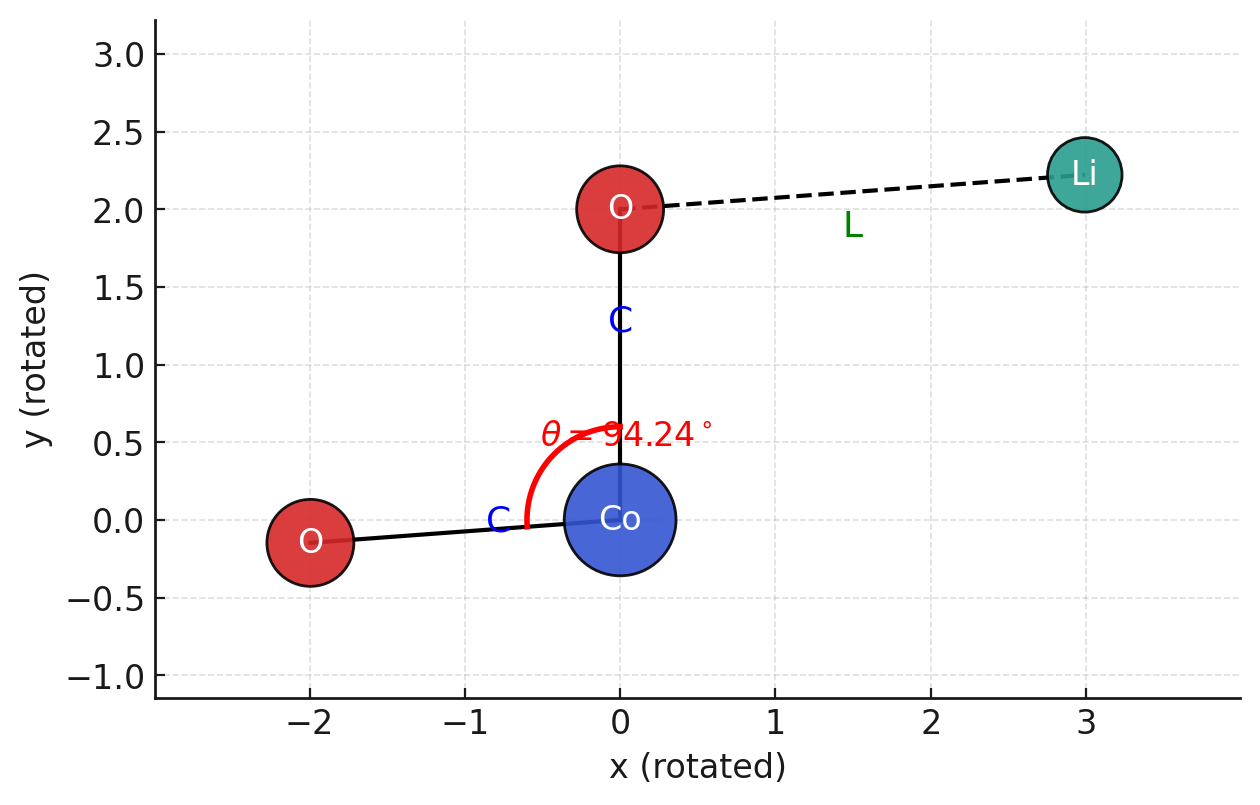
\includegraphics[width=0.6\textwidth]{Line Chart.png}
  \caption{LiCoO2 분자의 기하 구조}
  \label{fig:molecule}
\end{figure}
\begin{CodeBox}[title={Example: Python snippet}]
basis = 'sto3g'
# Slater Determinant의 한 원소가 되는 원자의 파동함수를 기술하기 위한 basis
# 여기서는 STO-3G 사용 
settings.use_pauli_sum_op = False
# 파울리스트링으로 헤밀토니안을 표현할때 SparsePauliOp의 형태가 아닌, 파울리 스트링의 합으로써 지정할것인가의 유무
# 구버전 Qiskit에서는 이러한 형태를 사용. 

# x = 1
C = 1.9220
# Co-O 의 평균 결합거리
L = 2.0946
# O-Li 의 평균 결합거리
theta = np.deg2rad(94.24)
# O-Co-O 결합각을 라디안 단위로 변경
# Co-O-Li 결합각의 경우, Symmetry 하도록 배치 
""" 
서로다른 x(산화상태)에 대응되는 결합거리, 결합각 을 정의 
다른 계산에서는 아래의 값중에서 대응되는 다른값을 사용
# # x= 0.94
# C = 1.9210
# L = 2.0944
# theta = np.deg2rad(94.27)

# #x = 0.78
# C = 1.9132
# L = 2.07
# theta = np.deg2rad(94.72)

# #x = 0.75
# C = 1.9059
# L = 2.07
# theta = np.deg2rad(95.07)
"""

Co = (0,0,0)
O_1 = (C,0,0)
O_2 = (C*np.cos(theta),C*np.sin(theta),0)
Li = (C+L*np.cos(np.pi-theta),-L*np.sin(np.pi-theta),0)

# Fig 1과 같이 결합각과 결합거리를 이용하여 분자의 기하학적인 구조를 정의. 
\end{CodeBox} 

\newpage

\subsection{Dimer 에너지 계산}
\begin{CodeBox}[title={Example: Python snippet}]
molecule_name = 'Li-O'
# 이후 편의설정을 위해 분자의 구성 정의(현재는 사용하지 않음)
O_Li_dimer_atoms = ["O", "Li"]
# Dirver를 구성하기 위한 원자 구성 정의
O_Li_dimer_coords = [O_1, Li]
# driver를 구성하기 위한 각 원자의 좌표 정의 
# 위에서 정의한 것을 바탕으로 (x,y,z) 좌표 사용 
O_Li_dimer_charge = 0
# Dimer의 전하량 정의
O_Li_dimer_multiplicity = 2
# Dimer 의 multiplicity(Singlet, Doublet,...) 정의. 이경우 Doublet
O_Li_moleculeinfo = MoleculeInfo(O_Li_dimer_atoms, O_Li_dimer_coords, charge=O_Li_dimer_charge, multiplicity=O_Li_dimer_multiplicity)
# 위의 정보들을 바탕으로 MoleculeInfo를 통해 분자의 정보 정의
driver = PySCFDriver.from_molecule(O_Li_moleculeinfo, basis=basis)
E_problem = driver.run()
# MoleculeInfo를 통해 PySCF에서 계산되어있는 정보를 가져온다.
num_spatial_orbitals = E_problem.num_spatial_orbitals
# Dimer의 공간오비탈 수 
num_particles = E_problem.num_particles
# Dimer의 전자수 
# 위 두가지 정보는 ActiveSpaceTransformer를 잘 정의하기 위함. 
as_transformer = ActiveSpaceTransformer((3,2), 4)
# 원자의 오비탈 배치를 기반으로 ActiveSpace 를 정의하여 ActiveSpaceTransformer정의
# ActiveSpace 를 지정하는 방식은 다음과 같다 
# ((up-spin 전자수, down-spin 전자수), 사용할 공간오비탈 수)
as_problem = as_transformer.transform(E_problem)
# 정의한 ActiveSpaceTransformer 를 바탕으로 새로운 problem을 정의
energy_arr, ansatz_order, opt_order = least_Energy(as_problem)
# 새로운 problem을 앞서 정의한 least_Energy함수에 집어넣어 에너지 계산 
print(energy_arr)
for k in range(len(energy_arr)):
    e=energy_arr[k]
    if e == np.min(energy_arr):
        print('optimal_calc :')
        print('anstaz: ', ansatz_order[k])
        print('optimizer: ', opt_order[k])
        print('Energy: ', e)
# 총 6개의 에너지가 담겨있는 리스트에서, 
# 에너지가 가장 작을때의 값과, 그떄의 Ansatz, Optimizer에 대한 정보를 Print한다. 

O_Li_dimer_energy=e
# 그리고 그 가장 작은 에너지를 해당 Dimer에서의 계산결과로 사용하기위해 새로운 변수로 정의한다. 
\end{CodeBox} 

Dimer 에너지 계산 코드에서 맨위의 기하학적인 구조를 통해 MoleculeInfo를 정의하는 부분과 각 Dimer의 Acivespace 를 정의해주는 부분만 옵션을 바꿔가며 총 6번(Dimer의 개수) 위 계산을 반복한다. 아래는 다른 Li-O 에 대응되는 코드이다. 
\begin{CodeBox}[title={Example: Python snippet}]
molecule_name = 'Li~O'
O_Li_dimer_atoms = ["O", "Li"]
O_Li_dimer_coords = [O_2, Li]
O_Li_dimer_charge = 0
O_Li_dimer_multiplicity = 4
O_Li_moleculeinfo = MoleculeInfo(O_Li_dimer_atoms, O_Li_dimer_coords, charge=O_Li_dimer_charge, multiplicity=O_Li_dimer_multiplicity)
"""
(중략)
"""
as_transformer = ActiveSpaceTransformer((4,1), 4)

\end{CodeBox} 

\subsection{FMO 계산}

\begin{CodeBox}[title={Example: Python snippet}]
dimer_energy_arr = [O_Li_dimer_energy,O_Li_2_dimer_energy,Co_O_1_dimer_energy,Co_O_2_dimer_energy,O_O_dimer_energy,Co_Li_dimer_energy]
#각 Dimer에 대한 에너지들로 이루어진 리스트
#각 성분은 각 Dimer 계산에서 6개의 Ansatz와 Optimizer의 조합중 가장 작은 에너지에 대응된다. 

O_mon= -74.78751
Co_mon = -1381.35417
Li_mon = -7.43241
# Monomer 에너지는 기하학적인 구조별로 다르지 않으므로 
# 한번 계산하여 미리 계산된 정보를 활용한다. 

FMO_VQE_energy = np.sum(dimer_energy_arr) - 2*(O_mon+Co_mon+Li_mon+O_mon)
# FMO 계산의 정의를 통해 Dimer 에너지의 합에서 Monomer에너지를 (N-2)번 빼주게 된다. 
# 여기서 N 은 Fragment의 개수로, 이번 경우에는 4

print(dimer_energy_arr)
# 결과 저장을 위해 dimer_energy_arr를 프린트

print("FMO_VQE_energy", FMO_VQE_energy)
# 결과 저장을 위해 최종 결과인 FMO_VQE_energy 를 프린트
\end{CodeBox} 


\end{document}